\documentclass[twoside,11pt,openany]{book}
\setcounter{tocdepth}{4}
\setcounter{secnumdepth}{4}

% Fix copy/pasting of ligatures in Acrobat
\input{glyphtounicode.tex}
\pdfgentounicode=1 %

\usepackage{etoolbox}

\input{preamble}

% All registers are named here. That way when we rename one we'll get errors if
% there are still references to the old name.

\usepackage{makeidx}
\makeindex

\usepackage{xspace}
\newcommand{\defregname}[2]{\providecommand{#1}{{\tt #2}\xspace}}
\newcommand{\deffieldname}[2]{\providecommand{#1}{{$|#2|$}\xspace}}
\deffieldname{\FcsrMstatusMprv}{MPRV}
\deffieldname{\FcsrMstatusMie}{MIE}
\deffieldname{\FcsrSstatusSie}{SIE}
\deffieldname{\Fmxl}{MXL}
\defregname{\Rmisa}{misa}
\defregname{\Rmtime}{mtime}
\defregname{\Rtime}{time}
\defregname{\Rmstatus}{mstatus}
\defregname{\Rsstatus}{sstatus}
\defregname{\Rvsstatus}{vsstatus}
\defregname{\Rmcause}{mcause}
\defregname{\Rmie}{mie}
\defregname{\Rxepc}{xepc}
\defregname{\Rmepc}{mepc}
\defregname{\Rmedeleg}{medeleg}
\defregname{\Rhedeleg}{hedeleg}
\defregname{\Rmstateenzero}{mstateen0}
\defregname{\Rhstateenzero}{hstateen0}

\deffieldname{\Fasid}{ASID}
\defregname{\Rsatp}{satp}
\defregname{\Rvsatp}{vsatp}

\defregname{\Azero}{a0}
\defregname{\Aone}{a1}

\defregname{\Rzero}{zero}
\defregname{\Szero}{s0}
\defregname{\Sone}{s1}

\defregname{\Tzero}{t0}

\defregname{\Xzero}{x0}
\defregname{\Xone}{x1}
\defregname{\Xeight}{x8}
\defregname{\Xnine}{x9}
\defregname{\Xten}{x10}
\defregname{\Xeleven}{x11}
\defregname{\Xthirtyone}{x31}
\defregname{\Fone}{f1}
\defregname{\Rpc}{pc}
\defregname{\Rmhartid}{mhartid}
\defregname{\Rdataone}{data1}

\input{hwbp_registers.tex.inc}
\input{core_registers.tex.inc}
\input{jtag_registers.tex.inc}
\input{dm_registers.tex.inc}
\input{sample_registers.tex.inc}
\input{abstract_commands.tex.inc}
\input{sw_registers.tex.inc}

\deffieldname{\Fhartsel}{\hyperref[hartsel]{hartsel}}
\deffieldname{\Fsize}{\hyperref[sizelo]{size}}
\deffieldname{\Faction}{action}
\deffieldname{\Fresethaltreq}{\hyperref[resethaltreq]{resethaltreq}}
\deffieldname{\Fkeepalive}{\hyperref[keepalive]{keepalive}}

\input{vc.tex}

\newcommand{\versionnum}{1.0.0\ifrelease\else-\releasename\fi}

\begin{document}

\title{RISC-V Debug Support\\
Version \versionnum\\
\GITHash
}
\author{Editors: \\
Paul Donahue \textless pdonahue@ventanamicro.com\textgreater, Ventana Micro Systems \\
Tim Newsome \textless tim@sifive.com\textgreater, SiFive, Inc.}
\date{\GITAuthorDate}
\maketitle

\markboth{RISC-V Debug Support Version \versionnum}
{RISC-V Debug Support Version \versionnum}
\thispagestyle{empty}

\frontmatter

\chapter{Preface}

{\bf Warning! This draft specification will change before being accepted as
standard, so implementations made to this draft specification will likely not
conform to the future standard.}


\tableofcontents
\listoffigures
\listoftables

\mainmatter

\newpage

\chapter{Introduction}
\label{sec:intro}

When a design progresses from simulation to a hardware implementation, a users's
control and understanding of the system's current state drops dramatically.
To help bring up and debug low level software and hardware,
it is critical to have good debugging support built into the hardware.
When a robust OS is running on a core, software can handle many
debugging tasks. Howevever, in many scenarios, hardware support is essential.

This document outlines a standard architecture for external debug support 
on RISC-V platforms. This architecture allows a variety of implementations and
tradeoffs, which is complementary to the wide range of RISC-V implementations.
At the same time, this specification defines common interfaces to
allow debugging tools and components to target a variety of platforms based on the RISC-V ISA.

System designers may choose to add additional hardware debug support,
but this specification defines a standard interface for common
functionality.

\section{Terminology}

A \emph{platform} is a single integrated circuit consisting of one or more
\emph{components}. Some components may be RISC-V cores, while others may have a different
function. Typically they will all be connected to a single system bus.
A single RISC-V core contains one or more hardware threads, called
\emph{harts}.

\section{About This Document}

\subsection{Structure}

This document contains two parts. The main part of the document is the
specification, which is given in the numbered sections. The second part
of the document is a set of  appendices. The information
in the appendix is intended to clarify and provide examples, but is
not part of the actual specification.


\subsection{Register Definition Format}

All register definitions in this document follow the format shown in Section~\ref{shortname}.
A simple graphic shows which fields are in the register. The
upper and lower bit indices are shown to the top left and top right of each
field. The total number of bits in the field are shown below it.

After the graphic follows a table which for each field lists its name,
description, allowed accesses, and reset value. The allowed accesses are listed
in Table~\ref{tab:access}.

\begin{table}[htp]
    \centering
    \caption{Register Access Abbreviations}
    \label{tab:access}
    \begin{tabulary}{\textwidth}{|l|L|}
        \hline
        R & Read-only. \\
        \hline
        R/W & Read/Write. \\
        \hline
        R/W0 & Read/Write. Only writing 0 has an effect.  \\
        \hline
        R/W1 & Read/Write. Only writing 1 has an effect.  \\
        \hline
        W & Write-only. When read this field returns 0. \\
        \hline
        W1 & Write-only. Only writing 1 has an effect. \\
        \hline
    \end{tabulary}
\end{table}

\input{sample_registers.tex}

%\section{Reading Order}

This section describes the minimal parts of the spec required to understand a
given piece of functionality. It's still best to read the whole thing, but it
might help you get started better than reading it all start to finish. No
matter what you want to learn about, it's best to read Section~\ref{overview}
first.

\subsubsection{Halt/Resume}

Sections \ref{dmi}, \ref{selectingharts}, \ref{haltcontrol}, \ref{dmcontrol}, \ref{dmstatus},
\ref{haltsum}, \ref{deb:halt}.

\subsubsection{Abstract Register Access}

Sections \ref{abstractcommands}, \ref{abstractcs}, \ref{command},
\ref{data0}, \ref{deb:abstractreg}.

\subsubsection{Program Buffer}

Sections \ref{programbuffer}, \ref{progbufcs}, \ref{progbuf0}, \ref{access
register}, \ref{debugmode}, \ref{deb:regprogbuf}, \ref{deb:mrprogbuf}.

\subsubsection{JTAG Debug Transport Module}

Sections \ref{dtm}, \ref{jtagdtm}, \ref{dbusaccess}.

\subsubsection{System Bus Access}

Sections \ref{systembusaccess}, \ref{sbcs}, \ref{sbaddress0}, \ref{sbaddress1},
\ref{sbaddress2}, \ref{sbdata0}, \ref{sbdata1}, \ref{sbdata2}, \ref{sbdata3},
\ref{deb:mrsysbus}.

\subsubsection{Reset}

TODO

\subsubsection{Security}

TODO

\subsubsection{Triggers}

TODO

\subsubsection{Serial Ports}

TODO



\chapter{System Overview} \label{overview}

Figure~\ref{fig:overview} shows the main components of External Debug Support.
Blocks shown in dotted lines are optional. 

\begin{figure}
   \centering
   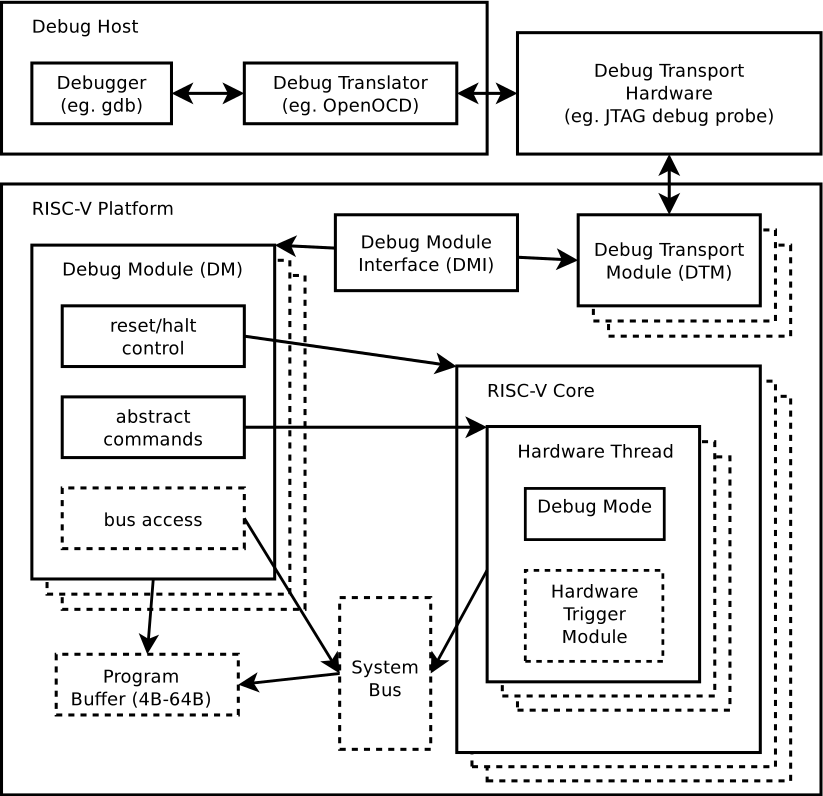
\includegraphics[width=\textwidth]{fig/overview-eps-converted-to.pdf}
   \caption{RISC-V Debug System Overview}
   \label{fig:overview}
\end{figure}

The user interacts with the Debug Host (eg. laptop), which is running a
debugger (eg. gdb).  The debugger communicates with a Debug Translator (eg.
OpenOCD, which may include a hardware driver) to communicate with Debug
Transport Hardware (eg.  Olimex USB-JTAG adapter).
The Debug Transport Hardware connects the Debug Host to the Platform's Debug
Transport Module (DTM).  The DTM provides access to the Debug Module (DM) using
the Debug Module Interface (DMI).

The DM allows the debugger to halt any hart in the platform. Abstract commands
provide access to GPRs.
The optional Program Buffer allows the debugger to execute arbitrary code on the hart,
which allows access to additional hart state. Alternatively, additional
abstract commands can provide access to additional hart state.

Each RISC-V hart may implement a Trigger Module. When trigger conditions
are met, harts will halt spontaneously and inform the debug module that they have
halted.

An optional system bus access block allows memory accesses without using a
RISC-V hart to perform the access.

Optional serial port blocks allow the Debug Transport to be re-used as a
generic communication interface.


\chapter{Debug Module (DM)} \label{dm}

\begin{steps}{The Debug Module is the interface between specific debug
    operations and their implementation. It might support the following
    operations:}
\item Provide access to a reset signal that allows debugging out of reset.
    (Required)
\item Allow any individual hart to be halted and resumed. (Required)
\item Provide status on which harts are halted. (Required)
\item Provide read and write access to a halted hart's GPRs. (Required)
\item Give the debugger necessary information about the implementation. (Required)
\item Provide access to other hart registers. (Optional)
\item Force the hart to execute arbitrary instructions. (Optional)
\item Allow multiple harts to be halted, resumed, and/or reset at the same time (Optional)
\end{steps}

A single DM can debug up to 1024 harts.

\section{Debug Module Interface (DMI)} \label{dmi}

The Debug Module Interface can be a trivial bus with one master and one slave,
or use a more full-featured bus like TileLink or the AMBA Advanced Peripheral
Bus. The details are left to the system designer.

The DMI uses between 7 and 32 address bits.  It supports read and write
operations, which may return an error. (Errors are only returned by the optional
System Bus Access and Serial Port blocks). The bottom of the address space is
used for the DM. Extra space can be used for custom debug devices, other cores,
additional DMs, etc.

\begin{table}[htp]
    \centering
    \caption{Debug Module Interface Address Space}
    \label{tab:header}
    \begin{tabulary}{\textwidth}{|r|L|}
        \hline
        0x00 -- 0x3f & Registers described in Section~\ref{dmdebbus}. \\
        \hline
        0x40 -- 0x5f & There are 1024 bits here, one for each hart that may
        exist in the system. If the hart is halted, the bit is 1.  Otherwise
        the bit is 0. The bit for hart 0 is the LSB in the 32-bit word at 0x40.
        The bit for hart 1023 is the MSB in the 32-bit word at 0x5f. \\
        \hline
    \end{tabulary}
\end{table}

\section{Reset Control} \label{reset}

This block is connected to a global reset signal, which can
reset, or hold in reset, every component in the platform,
except for the Debug Module and Debug
Transport Modules. The purpose of this feature is to allow debugging
programs from the first instruction executed, so exactly what is affected
by this reset is implementation dependent. Debug Module's own state and registers are
generally reset at power-up and if and only if
\Fdmactive in \Rdmcontrol is 0. This means that the halt state of all harts is
maintained provided that \Fdmactive is 1, although trigger CSRs may be cleared.

\section{Selecting Harts} \label{selectingharts}

Up to 1024 harts can be connected to the DM. The debugger can select any hart
by writing its index to \Fhartsel. Hart indexes start at 0 and are continuous
until the final index. This allows the debugger to enumerate all the harts
attached to the DM by trying each index until \Fanynonexistent is 1.

\section{Halt Control} \label{haltcontrol}

This block controls halt signals from the Debug Module to a hart.  It is used
to halt a hart, and let it run again.

To control halting and resuming, there are \Fhaltreq and \Fresumereq bits in
\Rdmcontrol.  When a debugger wants to halt a hart, it sets \Fhaltreq, waits
for \Fallhalted to indicate the hart is halted, and clears \Fhaltreq.  To
resume, the debugger sets \Fresumereq, waits for \Fallrunning to indicate the
hart is running, and clears \Fresumereq.

The Debug Module conceptually has a direct connection to the halt signal of
every hart that has a halt signal. When set or cleared, a hart must respond in
less than one second.  (How this is implemented is not further specified. A few
clock cycles will be a more typical latency.)

\section{Hart Array Mask Register} \label{hamask}

TODO: Write this section.

\section{Abstract Commands} \label{abstractcommands}

The DM supports a set of abstract commands, which a debugger can execute by
writing the command to \Rcommand.  If the command takes arguments, the debugger
must write them to the {\tt data} registers before writing to \Rcommand. If a
command returns results, they are placed in the {\tt data} registers when the
command is complete. Which {\tt data} registers are used for the arguments is
described in Table~\ref{tab:datareg}.  In all cases the least-significant word
is placed in the lowest-numbered {\tt data} register.  Depending on the
implementation, it may be possible to perform abstract commands even when the
hart is not halted.

\begin{table}[htp]
    \centering
    \caption{Use of Data Registers}
    \label{tab:datareg}
    \begin{tabulary}{\textwidth}{|r|l|l|l|}
        \hline
        XLEN & arg0/return value & arg1 & arg2 \\
        \hline
        32 & \Rdatazero & \Rdataone & \Rdatatwo \\
        \hline
        64 & \Rdatazero, \Rdataone & \Rdatatwo, \Rdatathree & \Rdatafour, \Rdatafive \\
        \hline
        128 & \Rdatazero--\Rdatathree & \Rdatafour--\Rdataseven & \Rdataeight--\Rdataeleven \\
        \hline
    \end{tabulary}
\end{table}

\begin{table}[htp]
    \centering
    \caption{Abstract Register Numbers}
    \label{tab:regno}
    \begin{tabulary}{\textwidth}{|r|l|}
        \hline
        0x0000 -- 0x0fff & CSRs \\
        \hline
        0x1000 -- 0x101f & GPRs \\
        \hline
        0x1020 -- 0x103f & Floating point registers \\
        \hline
        0xc000 -- 0xffff & Reserved for non-standard extensions and internal
        use. \\
        \hline
    \end{tabulary}
\end{table}

\input{abstract_commands.tex}


\begin{figure}
   \centering
   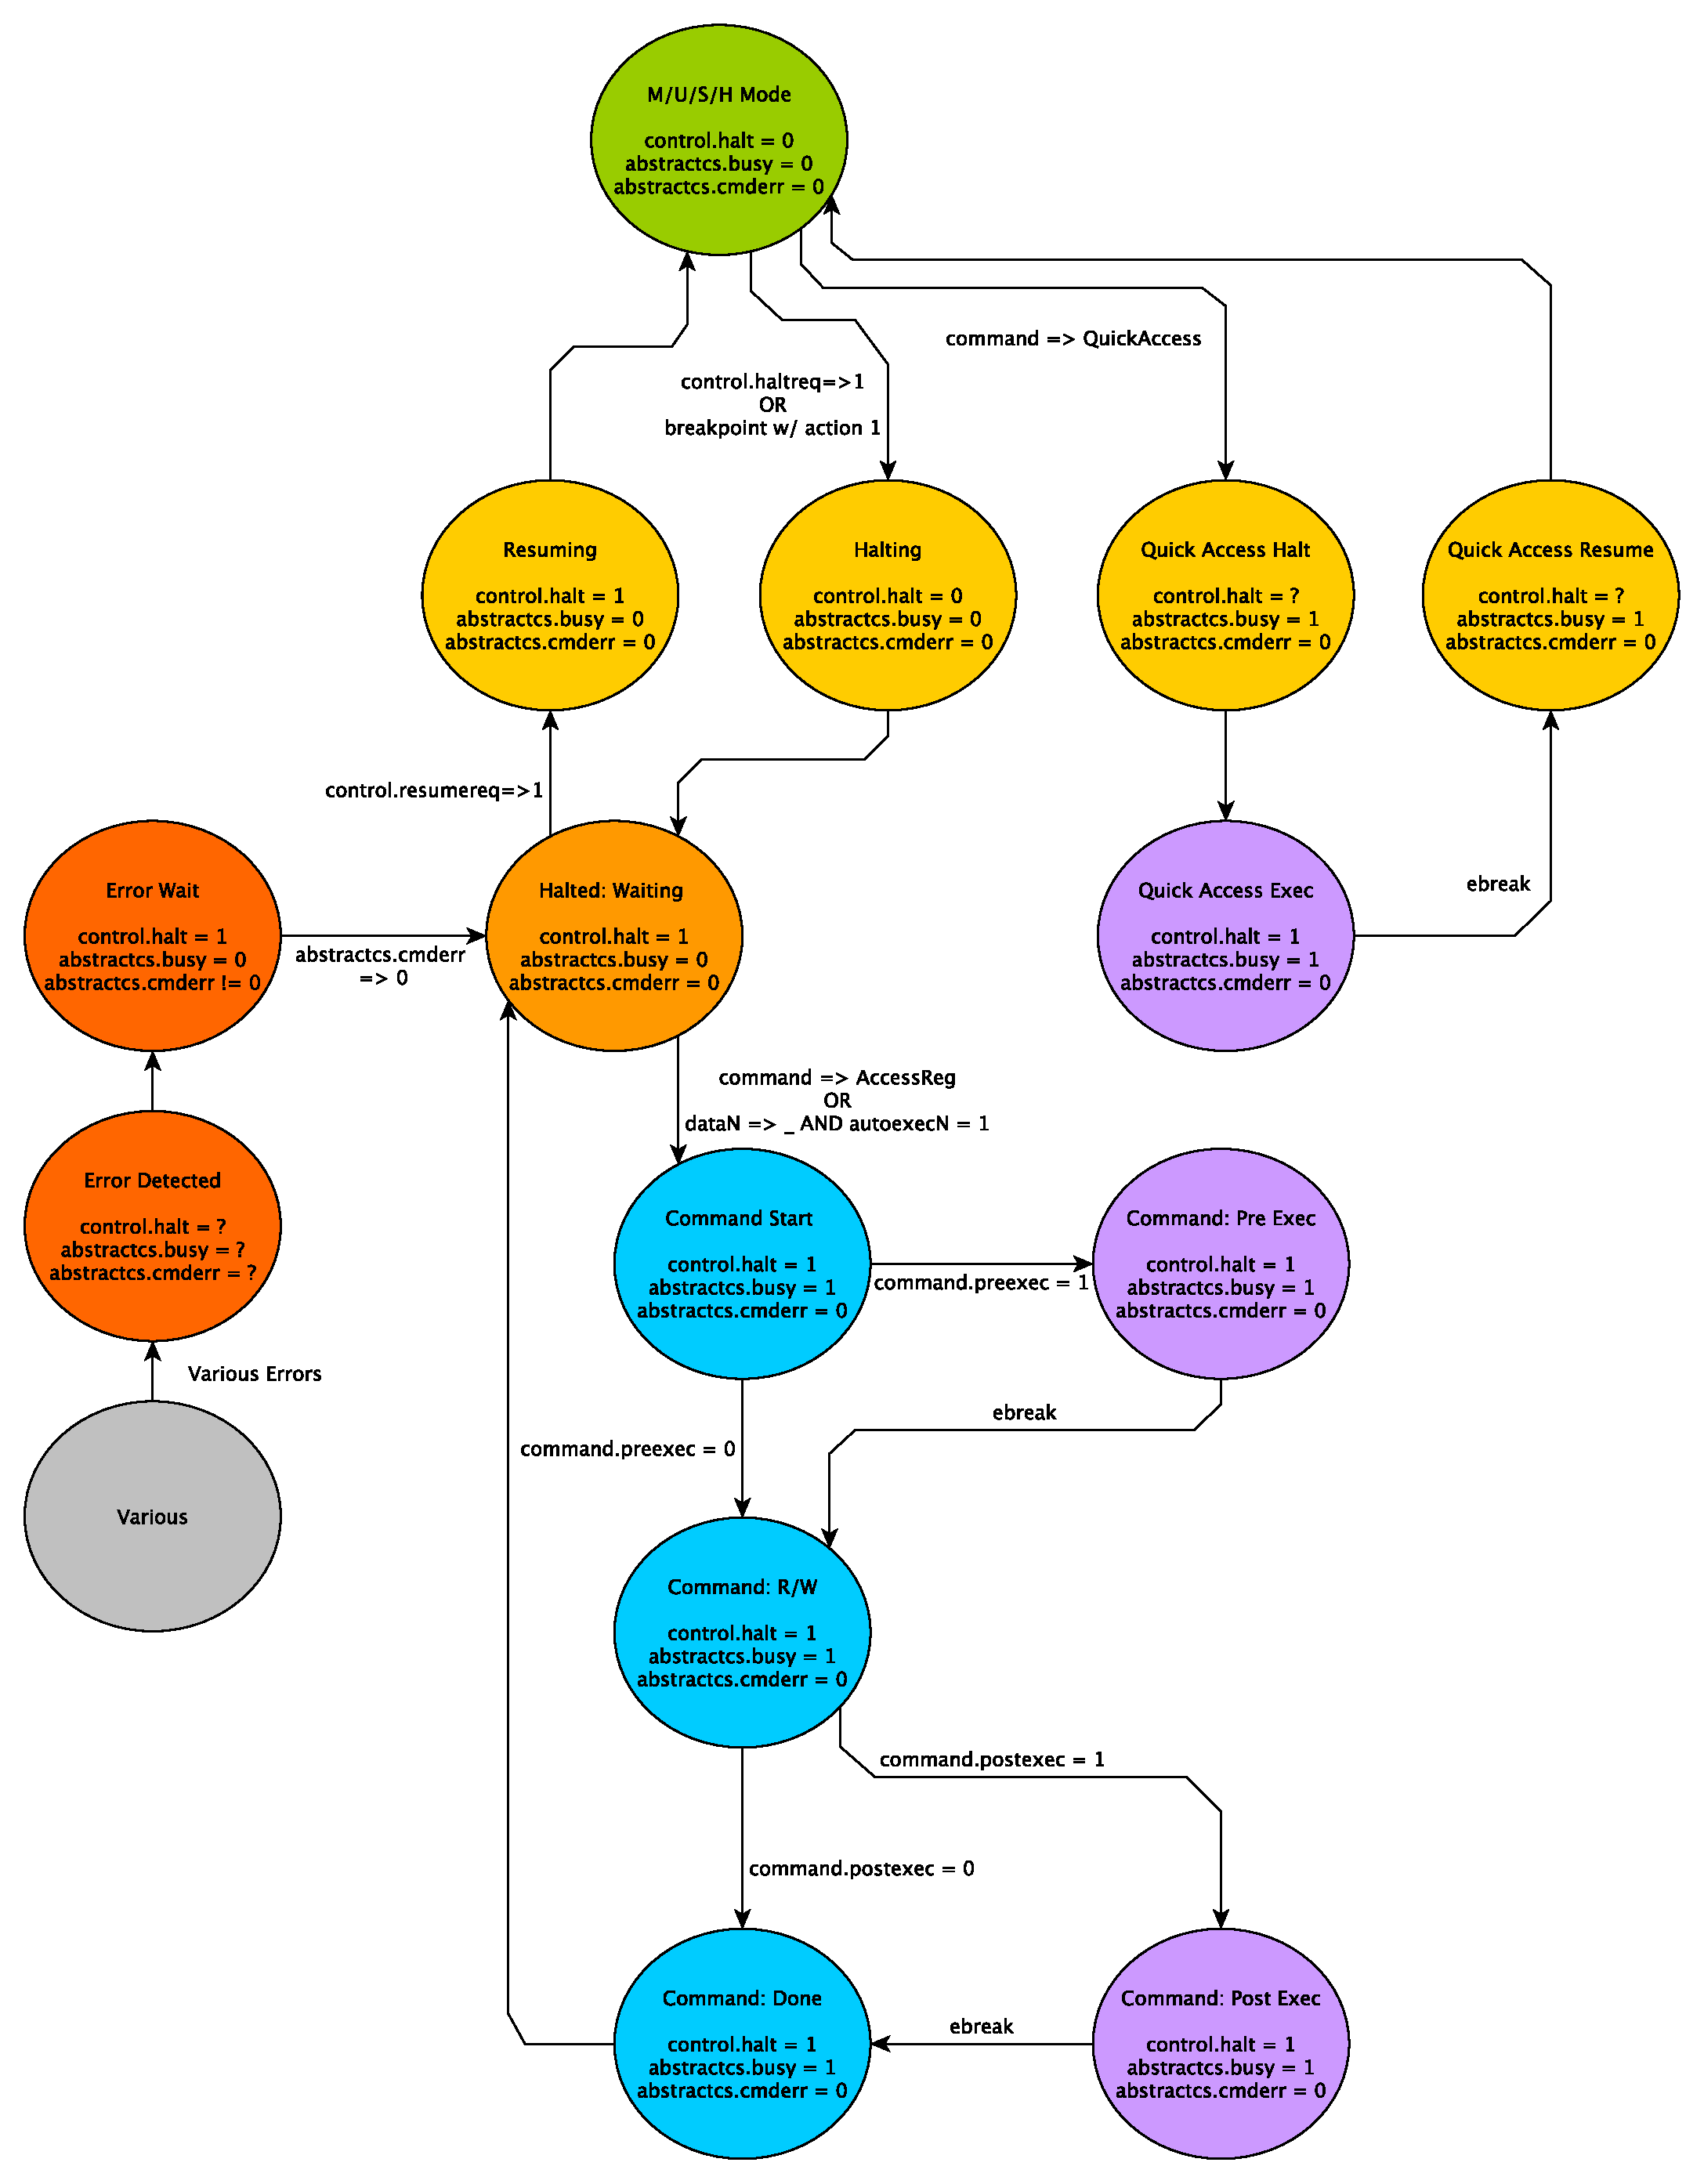
\includegraphics[width=\textwidth]{fig/abstract_commands.pdf}
   \caption[Run/Halt Debug State Machine]{Run/Halt Debug State Machine.
     As only a small amount of state is visibile to the debugger,
     the states and transitions are conceptual.}
   \label{fig:abstract_sm}
\end{figure}

Figure~\ref{fig:abstract_sm} shows a conceptual view of the states
passed through by a hart during run/halt debugging as influenced
by the different fields of \Rcommand.

\section{Program Buffer} \label{programbuffer}

To support executing arbitrary instructions on a halted hart, there may be a
Program Buffer that a debugger can write small programs to. Systems that don't
need any access beyond the abstract commands described in
Section~\ref{abstractcommands} may choose to omit this functionality.

A debugger can write a small program to the optional Program Buffer, and then
execute it exactly once using the \Fpreexec or \Fpostexec bits in \Rcommand.
If \Fprogsize is 1, the Program Buffer may only hold a single instruction.
This can be a 32-bit
instruction, or a compressed instruction in the lower 16 bits accompanied by a
compressed {\tt nop} in the upper 16 bits.  If \Fprogsize is greater than 1,
the debugger can write whatever program it likes, but the program must end with
{\tt ebreak} or {\tt ebreak.c}.

While these programs are executed, the hart does not leave Debug Mode (see
Section~\ref{debugmode}).  If an exception is encountered during execution of
the Program Buffer, no more instructions are executed, the hart remains in Debug
Mode, and \Fcmderr is set to 3.

Executing the Program Buffer may clobber \Rdpc. If that is the case, it must be
possible to read/write \Rdpc using an abstract command. The debugger must
attempt to save \Rdpc between halting and executing a Program Buffer, and then
restore \Rdpc before leaving Debug Mode.

\begin{commentary}
    Allowing Program Buffer execution to clobber \Rdpc allows for direct
    implementations that don't have a separate PC register, and do need to use
    the PC when executing the Program Buffer.
\end{commentary}

\section{System Bus Access} \label{systembusaccess}

When a Program Buffer is present, a debugger can access the system bus by having a
RISC-V hart perform the accesses it requires.
An alternative is to implement a System Bus Access block.
The System Bus Access block uses physical addresses.

\begin{commentary}
Implementing a System Bus Access block has several benefits even
when a Debug Module also implements a Program Buffer. 
First, it is possible to
access memory in a running system with minimal impact.  Second, it may improve
performance when accessing memory.
Third, it may provide
access to devices that a hart does not have access to.
\end{commentary}

\section{Quick Access}

Some systems can only be halted very briefly. There are several mechanisms that
can still allow accessing resources in such a running system.

First, an implementation may implement abstract commands that work without
halting the hart.

Second, the Quick Access abstract command can be used to halt a hart, quickly
execute the contents of the Program Buffer, and let the hart run again.
Combined with instructions that allow Program Buffer code to access the
{\tt data} registers, as described in \ref{hartinfo}, this can be used to quickly
perform a memory or register access. For some systems this will be too
intrusive, but many systems that can't be halted can bear an occasional hiccup
of a hundred or less cycles.

Third, if the System Bus Access block is implemented, it can be used while a
hart is running to access memory.

\section{Security}

To protect intellectual property it may be desirable to lock access to the
Debug Module.  To allow access during a manufacturing process and not
afterwards, a reasonable solution could be to add a fuse bit to the Debug
Module that can be used to be permanently disable it. Since this is technology
specific, it is not further addressed in this spec.

Another option is to allow the DM to be unlocked only by users who have an
access key. A few bits in \Rdmstatus and \Rauthdata can support an arbitrarily
complex authentication mechanism.  When \Fauthenticated is clear, the DM must
not interact with the rest of the platform in any way.

\section{Serial Ports}

The Debug Module may implement up to 8 serial ports. They support basic flow
control and full duplex data transfer between a component and the debugger.
They can be used to communicate with a debug monitor running on a hart, for the
equivalent of printf debugging, to provide a simple CLI without requiring any
extra peripherals, or more generally to emulate devices that aren't present.
All these uses require software support, and are not further specified here.

\section{Debug Module DMI Registers} \label{dmdebbus}

\input{dm1_registers.tex}

\section{Debug Module Serial Registers} \label{dmsysbus}

The Debug Module's serial port registers must be accessible from the
component memory space. The Debug Module's system bus registers  base address
is discoverable in the configuration string. The offsets from this base
are given in this section.

\input{dm2_registers.tex}

\chapter{Sdext ISA Extension}
\label{sec:core_debug}

This chapter describes the Sdext ISA extension. It must be implemented to make
external debug work, and is only useful in conjunction with external debug.

Modifications to the RISC-V core to support debug are kept to a minimum.  There
is a special execution mode (Debug Mode) and a few extra CSRs. The DM takes care
of the rest.

In order to be compatible with this specification an implementation must
implement everything described in this section that is not explicitly listed as
optional.

\section{Debug Mode} \label{debugmode}

Debug Mode is a special processor mode used only when a hart is halted for
external debugging. Because the hart is halted, there is no forward progress in
the normal instruction stream.
How Debug Mode is implemented is not specified here.

\begin{steps}{When executing code due to an abstract command, the hart stays in
    Debug Mode and the following apply:}
\item All operations are executed with machine mode privilege, except that
    additional Debug Mode CSRs are accessible and
    \FcsrMstatusMprv in \Rmstatus may be ignored according to \FcsrDcsrMprven.
    Full permission checks, or a relaxed set of permission checks, will apply
    according to \FdmAbstractcsRelaxedpriv.
\item All interrupts (including NMI) are masked.
\item Exceptions don't update any registers.  That includes {\tt cause}, {\tt
    epc}, {\tt tval}, {\tt dpc}, and \Rmstatus. They do end execution of the
    Program Buffer.
\item No action is taken if a trigger matches.
\item If \FcsrDcsrStopcount is 0 then counters continue. If it is 1 then
    counters are stopped.
\item If \FcsrDcsrStoptime is 0 then \Rtime continues to update. If
    it is 1 then \Rtime will not update. It will resynchronize with
    \Rmtime after leaving Debug Mode.
\item The {\tt wfi} instruction acts as a {\tt nop}.
\item Almost all instructions that change the privilege mode have \unspecified\
    behavior.  This includes {\tt ecall}, {\tt mret}, {\tt sret}, and {\tt uret}.
    (To change the privilege mode, the debugger can write
    \FcsrDcsrPrv and \FcsrDcsrV in \RcsrDcsr). The only exception is {\tt ebreak}, which ends
    execution of the Program Buffer when executed.
\item All control transfer instructions may act as illegal instructions if
    their destination is in the Program Buffer. If one such instruction acts as
    an illegal instruction, all such instructions must act as illegal
    instructions.
\item All control transfer instructions may act as illegal instructions if
    their destination is outside the Program Buffer. If one such instruction
    acts as an illegal instruction, all such instructions must act as
    illegal instructions.
\item Instructions that depend on the value of the PC (e.g.\ {\tt auipc}) may act
    as illegal instructions.
\item Effective XLEN is DXLEN.
\item Forward progress is guaranteed.
\end{steps}

\begin{commentary}
    When \FcsrDcsrMprven=1, the external debugger can set MPRV and MPP appropriately to
    have hardware perform memory accesses with the appropriate endianness, address
    translation, permission checks, and PMP/PMA checks (subject to \FdmAbstractcsRelaxedpriv).
    This is also the only way to access all of physical memory when 34-bit physical
    addresses are supported on a Sv32 hart. If hardware ties \FcsrDcsrMprven to 0 then the
    external debugger is expected to simulate all the effects of MPRV, including
    any extensions that affect memory accesses.
    For these reasons it is recommended to tie \FcsrDcsrMprven to 1.
\end{commentary}

\section{Load-Reserved/Store-Conditional Instructions}

The reservation registered by an {\tt lr} instruction on a memory address may
be lost when entering Debug Mode or while in Debug Mode.  This means that there
may be no forward progress if Debug Mode is entered between {\tt lr} and {\tt
sc} pairs.

\begin{commentary}
    This is a behavior that debug users must be aware of. If they have a
    breakpoint set between a {\tt lr} and {\tt sc} pair, or are stepping
    through such code, the {\tt sc} may never succeed.  Fortunately in general use
    there will be very few instructions in such a sequence, and anybody
    debugging it will quickly notice that the reservation is not occurring.
    The solution in that case is to set a breakpoint on the first instruction
    after the {\tt sc} and run to it. A higher level debugger may choose to
    automate this.
\end{commentary}

\section{Wait for Interrupt Instruction}

If halt is requested while {\tt wfi} is executing, then the hart must leave the
stalled state, completing this instruction's execution, and then enter Debug
Mode.

\section{Single Step}

\subsection{Step Bit In Dcsr} \label{stepBit}

This method is only available to external debuggers, and is the preferred way
to single step.

An external debugger can cause a halted hart to execute a single instruction or
trap and then re-enter Debug Mode by setting \FcsrDcsrStep before resuming.  If
\FcsrDcsrStep is set when a hart resumes then it will single step, regardless
of the reason for resuming.

If control is transferred to a trap handler while executing the instruction,
then Debug Mode is re-entered immediately after the PC is changed to the trap
handler, and the appropriate {\tt tval} and {\tt cause} registers are updated.
In this case none of the trap handler is executed, and if the cause was a
pending interrupt no instructions might be executed at all.

If executing or fetching the instruction causes a trigger to fire with action=1, Debug Mode
is re-entered immediately after that trigger has fired. In that case \FcsrDcsrCause is
set to 2 (trigger) instead of 4 (single step).  Whether the instruction is
executed or not depends on the specific configuration of the trigger.

If the instruction that is executed causes the PC to change to an address where
an instruction fetch causes an exception, that exception does not occur until
the next time the hart is resumed. Similarly, a trigger at the new address does
not fire until the hart actually attempts to execute that instruction.

If the instruction being stepped over is {\tt wfi} and would normally stall the
hart, then instead the instruction is treated as {\tt nop}.

\subsection{Icount Trigger}

Native debuggers won't have access to \RcsrDcsr, but can use the \RcsrIcount
trigger by setting \FcsrIcountCount to 1.

\begin{steps}{This approach does have some limitations:}
    \item Interrupts will fire as usual. Debuggers that want to disable
        interrupts while stepping must disable them by changing \Rmstatus, and
        specially handle instructions that read \Rmstatus.
    \item {\tt wfi} instructions are not treated specially and might take a
        very long time to complete.
\end{steps}

This mechanism cleanly supports a system which supports multiple privilege
levels, where the OS or a debug stub runs in M-Mode while the program being
debugged runs in a less privileged mode. Systems that only support M-Mode can
use \RcsrIcount as well, but count must be able to count several instructions
(depending on the software implementation). See Section \ref{nativestep}.

\section{Reset}

If the halt signal (driven by the hart's halt request bit in the Debug Module)
or \Fresethaltreq are asserted when a hart comes out of reset, the hart must
enter Debug Mode before executing any instructions, but after performing any
initialization that would usually happen before the first instruction is
executed.

\section{Resume}

\begin{steps}{When a hart resumes:}
    \item \Rpc changes to the value stored in \RcsrDpc.
    \item The current privilege mode and virtualization mode are changed to that specified by
        \FcsrDcsrPrv and \FcsrDcsrV.
    \item If the new privilege mode is less privileged than M-mode,
        \FcsrMstatusMprv in \Rmstatus is cleared.
    \item The hart is no longer in debug mode.
\end{steps}

\section{XLEN}

While in Debug Mode, XLEN is DXLEN. It is up to the debugger to determine the
XLEN during normal program execution (by looking at \Rmisa) and to clearly
communicate this to the user.

\section{Core Debug Registers} \label{debreg}

The supported Core Debug Registers must be implemented for each hart that can
be debugged. They are CSRs, accessible using the RISC-V {\tt csr} opcodes and
optionally also using abstract debug commands.

Attempts to access a non-existent Core Debug Register raise an illegal
instruction exception.

\input{core_registers.tex}

\section{Virtual Debug Registers} \label{virtreg}

\input{sw_registers.tex}

\chapter{Sdtrig ISA Extension}
\label{sec:trigger}

This chapter describes the Sdtrig ISA extension, which can be implemented
independently of functionality described in the other chapters. It consists
exclusively of the Trigger Module (TM).

Triggers can cause a breakpoint exception, entry into Debug Mode, or a trace action
without having to execute a special instruction. This makes them invaluable
when debugging code from ROM. They can trigger on execution of instructions at
a given memory address, or on the address/data in loads/stores.

A hart can be compatible with this specification without implementing any
trigger functionality at all, but if it is implemented then it must conform to
this section. If triggers aren't implemented, the CSRs must not exist at all and
accessing them results in an illegal instruction exception.

A trigger matches when the conditions that it specifies (e.g. a load from a
specific address) are met. A trigger fires when a trigger that matches performs
the action configured for that trigger.

Triggers do not fire while in Debug Mode.

\section{Enumeration}

\begin{steps}{Each trigger may support a variety of features. A debugger can
    build a list of all triggers and their features as follows:}
\item Write 0 to \RcsrTselect. If this results in an illegal instruction
    exception, then there are no triggers implemented.
\item Read back \RcsrTselect and check that it contains the written value. If not,
    exit the loop.
\item Read \RcsrTinfo.
\item If that caused an exception, the debugger must read \RcsrTdataOne to
    discover the type. (If \FcsrTdataOneType is 0, this trigger doesn't exist. Exit the
    loop.)
\item If \FcsrTinfoInfo is 1, this trigger doesn't exist. Exit the loop.
\item Otherwise, the selected trigger supports the types discovered in \FcsrTinfoInfo.
\item Repeat, incrementing the value in \RcsrTselect.
\end{steps}

\begin{commentary}
    The above algorithm reads back \RcsrTselect so that implementations which have
    $2^n$ triggers only need to implement $n$ bits of \RcsrTselect.

    The algorithm checks \RcsrTinfo and \FcsrTdataOneType in case the implementation has $m$
    bits of \RcsrTselect but fewer than $2^m$ triggers.
\end{commentary}

\section{Actions}

Triggers can be configured to take one of several actions when they fire.
Table~\ref{tab:action} lists all options.

\begin{table}[H]
\centering
\caption{\FcsrMcontrolAction encoding}
\label{tab:action}
\begin{tabular}{|r|L|}
\hline
Value & Description \\
\hline
0 & Raise a breakpoint exception. (Used when software wants to use the
    trigger module without an external debugger attached.)  \Rxepc
    must contain the virtual address of the next instruction that must
    be executed to preserve the program flow. \\
\hline
1 & Enter Debug Mode.
    \RcsrDpc must contain the virtual address of the next instruction that must
    be executed to preserve the program flow.

    This action is only legal when the trigger's \FcsrTdataOneDmode is 1.
    Since the {\tt tdata} registers are WARL, hardware should clear the action
    field whenever the action field is 1, the new value of \FcsrTdataOneDmode would be 0, and the
    new value of the action field would be 1. \\
\hline
2 & Trace on, described in the trace specification. \\
\hline
3 & Trace off, described in the trace specification. \\
\hline
4 & Trace notify, described in the trace specification. \\
\hline
5 & Reserved for use by the trace specification. \\
\hline
8 -- 9 & Signal the firing of the trigger to other blocks within the hart (e.g. as countable events to hpmcounters).  Use external debug trigger output 0 or 1 (respectively). \\
\hline
other & Reserved for future use. \\
\hline
\end{tabular}
\end{table}

\section{Priority}

Table~\ref{tab:priority} lists the synchronous exceptions from the Privileged
Spec, and where the various types of triggers fit in. The first 3 columns come
from the Privileged Spec, and the final column shows where triggers fit in.
Priorities in the table are separated by horizontal lines, so e.g. etrigger and
itrigger have the same priority.
If this table contradicts the table in the Privileged Spec, then the latter
takes precedence.

This table only applies if triggers are precise. Otherwise triggers
will fire some indeterminate time after the event, and the priority is
irrelevant.
When triggers are chained, the priority is the lowest priority of the triggers
in the chain.

\begin{table}[H]
\centering
\begin{tabular}{|l|r|l|l|}
  \hline
  Priority      & Exception & Description & Trigger \\
                &      Code &             & \\
  \hline
  {\em Highest} &          3 & & etrigger \\
                &          3 & & icount \\
                &          3 & & itrigger \\
                &          3 & & mcontrol/mcontrol6 after \\
                &            & & \hspace{2em}(on previous instruction) \\
                \hline
                &          3 & Instruction address breakpoint & mcontrol/mcontrol6 execute address before \\ \hline
                &         12 & Instruction page fault & \\ \hline
                &          1 & Instruction access fault & \\ \hline
                &          3 & & mcontrol/mcontrol6 execute data before \\ \hline
                &          2 & Illegal instruction & \\
                &          0 & Instruction address misaligned & \\
                &   8, 9, 11 & Environment call & \\
                &          3 & Environment break & \\
                &          3 & Load/Store/AMO address breakpoint & mcontrol/mcontrol6 load/store address before \\
                &          3 & & mcontrol/mcontrol6 store data before \\ \hline
                &          6 & Store/AMO address misaligned & \\
                &          4 & Load address misaligned & \\ \hline
                &         15 & Store/AMO page fault & \\
                &         13 & Load page fault & \\ \hline
                &          7 & Store/AMO access fault & \\
                &          5 & Load access fault & \\
  {\em Lowest}  &          3 & & mcontrol/mcontrol6 load data before \\
  \hline
\end{tabular}
\caption{Synchronous exception priority in decreasing priority order.}
\label{tab:priority}
\end{table}

When multiple triggers in the same priority fire at once, \FcsrMcontrolHit (if
implemented) is set for all of them.  If more than one of these triggers has
\FcsrMcontrolSixAction=0 then {\tt tval} is updated in accordance with one of
them, but which one is \unspecified.  If one of these triggers has
the ``enter Debug Mode'' action (1) and another
trigger has the ``raise a breakpoint exception'' action (0),
the preferred behavior is to have both actions take place.  It is
implementation-dependent which of the two happens first.  This ensures both
that the presence of an external debugger doesn't affect execution and that a
trigger set by user code doesn't affect the external debugger. If this is not
implemented, then the hart must enter Debug Mode and ignore the breakpoint
exception. In the latter case, \FcsrMcontrolHit of the trigger whose action is 0 must still
be set, giving a debugger an opportunity to handle this case. What happens with
trace actions when triggers with different actions are also firing is left to
the trace specification.

\section{Native Triggers}
\label{sec:nativetrigger}

Triggers can be used for native debugging when \FcsrMcontrolSixAction=0.
If supported by the hart and desired by the debugger, triggers will often be
programmed to have \FcsrMcontrolSixM=0 so that when they fire they cause a
breakpoint exception to trap to a more privileged mode. That breakpoint
exception can either be taken in M-mode or it can be delegated to a less
privileged mode. However, it is possible for triggers to fire in the same
mode that the resulting exception will be handled in.

In these cases such a trigger may cause a breakpoint exception while already
in a trap handler. This might leave the hart unable to resume normal execution
because state such as \Rmcause and \Rmepc would be overwritten.

\begin{commentary}
\begin{steps}{In particular, when \FcsrMcontrolSixAction=0:}
\item mcontrol and mcontrol6 triggers with \FcsrMcontrolSixM=1 can cause a
breakpoint exception that is taken from M-mode to M-mode (regardless of
delegation).
\item mcontrol and mcontrol6 triggers with \FcsrMcontrolSixS=1 can cause a
breakpoint exception that is taken from S-mode to S-mode if \Rmedeleg[3]=1.
\item mcontrol6 triggers with \FcsrMcontrolSixVs=1 can cause a
breakpoint exception that is taken from VS-mode to VS-mode if \Rmedeleg[3]=1
and \Rhedeleg[3]=1.
\item icount triggers with \FcsrIcountM=1 can cause a
breakpoint exception that is taken from M-mode to M-mode (regardless of
delegation).
\item icount triggers with \FcsrIcountS=1 can cause a
breakpoint exception that is taken from S-mode to S-mode if \Rmedeleg[3]=1.
\item icount triggers with \FcsrIcountVs=1 can cause a
breakpoint exception that is taken from VS-mode to VS-mode if \Rmedeleg[3]=1
and \Rhedeleg[3]=1.
\item etrigger and itrigger triggers will always be taken from a trap handler
before the first instruction of the handler.  If etrigger/itrigger is set to
trigger on exception/interrupt X and if X is delegated to mode Y then the
trigger will cause a breakpoint exception that is taken from mode Y to mode
Y unless breakpoint exceptions are delegated to a more privileged mode than Y.
\item tmexttrigger triggers are asynchronous and may occur in any mode and
at any time.
\end{steps}
\end{commentary}

\begin{steps}{Harts that support triggers with \FcsrMcontrolSixAction=0
should implement one of the following two solutions to solve the problem of
reentrancy:}
\item The hardware prevents triggers with \FcsrMcontrolSixAction=0 from
matching while in M-mode and while \FcsrMstatusMie in \Rmstatus is 0.  If
\Rmedeleg[3]=1 then it prevents triggers with \FcsrMcontrolSixAction=0
from matching while in S-mode and while \FcsrSstatusSie in \Rsstatus is 0.
If \Rmedeleg[3]=1 and \Rhedeleg[3]=1 then it prevents triggers with
\FcsrMcontrolSixAction=0 from matching while in VS-mode and while
\FcsrSstatusSie in \Rvsstatus is 0.
\item \FcsrTcontrolMte and \FcsrTcontrolMpte in \RcsrTcontrol is
implemented.  \Rmedeleg[3] is hard-wired to 0.
\end{steps}

\begin{commentary}
The first option has the limitation that interrupts might be disabled at
times when a user still might want triggers to fire.  It has the benefit
that breakpoints are not required to be handled in M-mode.

The second option has the benefit that it only disables triggers during
the trap handler, though it requires specific software support for this debug
feature in the M-mode trap handlers.  It can only work if breakpoints are not
delegated to less privileged modes and therefore targets primarily
implementations without S-mode.

Because \RcsrTcontrol is not accessible to S-mode, the second option can
not be extended to accommodate delegation without adding additional S-mode
and VS-mode CSRs.

Both options prevent etrigger and itrigger from having any effect on
exceptions and interrupts that are handled in M-mode.  They also prevent
triggering during some initial portion of each handler.  Debuggers should
use other mechanisms to debug these cases, such as patching the handler
or setting a breakpoint on the instruction after \FcsrMstatusMie is cleared.
\end{commentary}

\section{Trigger Registers}

These registers are CSRs, accessible using the RISC-V {\tt csr} opcodes and
optionally also using abstract debug commands.

Almost all trigger functionality is optional. All {\tt tdata} registers follow
write-any-read-legal semantics. If a debugger writes an unsupported
configuration, the register will read back a value that is supported (which may
simply be a disabled trigger).  This means that a debugger must always read
back values it writes to {\tt tdata} registers, unless it already knows already
what is
supported.  Writes to one {\tt tdata} register must not modify the contents of
other {\tt tdata} registers, nor the configuration of any trigger besides the
one that is currently selected.

The combination of these rules means that a debugger cannot simply set a
trigger by writing \RcsrTdataOne, then \RcsrTdataTwo, etc. The current value
of \RcsrTdataTwo might not be legal with the new value of \RcsrTdataOne. To
help with this situation, it is guaranteed that writing 0 to \RcsrTdataOne
disables the trigger, and leaves it in a state where \RcsrTdataTwo and
\RcsrTdataThree can be written with any value that makes sense for any
trigger type supported by this trigger.

\begin{steps}{As a result, a debugger can write any supported trigger as
follows:}
\item Write 0 to \RcsrTdataOne. (This will result in \RcsrTdataOne containing a
    non-zero value, since the register is \warl.)
\item Write desired values to \RcsrTdataTwo and \RcsrTdataThree.
\item Write desired value to \RcsrTdataOne.
\end{steps}

Code that restores CSR context of triggers that might be configured to fire in
the current privilege mode must use this same sequence to restore the triggers.
This avoids the problem of a partially written trigger firing at a different
time than is expected.

Attempts to access a non-existent Trigger Register raise an illegal instruction
exception.

\input{hwbp_registers.tex}

\chapter{Debug Transport Module (DTM)} \label{dtm}

Debug Transport Modules provide access to the DM over one or more transports
(eg. JTAG or USB).

There may be multiple DTMs in a single platform. Ideally every component that
communicates with the outside world includes a DTM, allowing a platform to be
debugged through every transport it supports.  For instance a USB component
could include a DTM. This would trivially allow any platform to be debugged
over USB. All that is required is that the USB module already in use also has
access to the Debug Module Interface.

Using multiple DTMs at the same time is not supported. It is left to the user
to ensure this does not happen.

This specification defines a JTAG DTM in Section~\ref{sec:jtagdtm}. Additional DTMs
may be added in future versions of this specification.

\section{JTAG Debug Transport Module} \label{sec:jtagdtm}

This Debug Transport Module is based around a normal JTAG Test Access Port
(TAP).  The JTAG TAP allows access to arbitrary JTAG registers by first
selecting one using the JTAG instruction register (IR), and then accessing it
through the JTAG data register (DR).

\subsection{JTAG Background}

JTAG refers to IEEE Std 1149.1-2013. It is a standard that defines test logic
that can be included in an integrated circuit to test the interconnections
between integrated circuits, test the integrated circuit itself, and observe or
modify circuit activity during the component's normal operation.
This specification uses the latter functionality.
The JTAG standard defines a Test Access Port (TAP) that
can be used to read and write a few custom registers, which can be used to
communicate with debug hardware in a component.

\subsection{JTAG DTM Registers}

JTAG TAPs used as a DTM must have an IR of at least 5 bits.
When the TAP is reset, IR must default to
00001, selecting the IDCODE instruction. A full list of JTAG registers along
with their encoding is in Table~\ref{dtmTable:jtagregisters}.
If the IR actually has more than 5 bits, then the encodings in
Table~\ref{dtmTable:jtagregisters} should be extended with 0's in their most
significant bits, except for the 0x1f encoding of BYPASS, which must be
extended with 1's in the most significant bits.
The only regular JTAG registers a debugger might use are BYPASS and IDCODE, but this
specification leaves IR space for many other standard JTAG instructions.
Unimplemented instructions must select the BYPASS register.

\input{jtag_registers.tex}

\subsection{JTAG Connector}

\subsubsection{Recommended JTAG Connector}

To make it easy to acquire debug hardware, this spec recommends a connector
that is compatible with the MIPI-10 .05 inch connector specification, as described
in MIPI Debug \& Trace Connector Recommendations, Version 1.20, 2 July 2021.

The connector has .05 inch spacing, gold-plated male header with .016 inch thick
hardened copper or beryllium bronze square posts (SAMTEC FTSH or equivalent).
Female connectors are compatible $20\mu m$ gold connectors.

Viewing the male header from above (the pins pointing at your eye), a target's
connector looks as it does in Table~\ref{tab:mipiten}.  The function of each pin
is described in Table~\ref{tab:pinout}.

\begin{table}[H]
    \centering
    \caption{MIPI 10-pin JTAG + nRESET Connector Diagram}
    \label{tab:mipiten}
    \begin{tabular}{|r|c|c|l|}
        \hline
        VREF DEBUG & 1 & 2 & TMS \\
        \hline
        GND & 3 & 4 & TCK \\
        \hline
        GND & 5 & 6 & TDO \\
        \hline
        GND or KEY & 7 & 8 & TDI \\
        \hline
        GND & 9 & 10 & nRESET \\
        \hline
    \end{tabular}
\end{table}

\begin{table}[htp]
    \centering
    \caption{JTAG Connector Pin Functions}
    \label{tab:pinout}
    \begin{tabulary}{\textwidth}{|c|L|}
      \hline
      VREF DEBUG & Reference voltage for logic high. \\
      \hline
      GND & Connected to ground. \\
      \hline
      TMS & JTAG TMS signal, driven by the debug adapter. \\
      \hline
      TCK & JTAG TCK signal, driven by the debug adapter. \\
      \hline
      TDO & JTAG TDO signal, driven by the target. \\
      \hline
      GND or KEY &
        This pin may be cut on the male and plugged on the female header to
        ensure the header is always plugged in correctly. It is, however,
        recommended to use this pin as an additional ground, to allow for
        fastest TCK speeds. A shrouded connector should be used to prevent the
        cable from being plugged in incorrectly. \\
      \hline
      TDI & JTAG TDI signal, driven by the debug adapter. \\
      \hline
      nRESET & Open drain active low reset signal, usually driven by the debug
        adapter.  The signal may be used bi-directional to drive or sense the
        target reset signal.

        Asserting reset should reset any RISC-V cores as well as any other
        peripherals on the PCB. It should not reset the debug logic.  This pin
        is optional but strongly encouraged.

        If necessary, this pin could be used as nTRST instead.

        nRESET should never be connected to the TAP reset, otherwise the
        debugger might not be able to debug through a reset to discover the
        cause of a crash or to maintain execution control after the reset. \\
      \hline
      RTCK & Return test clock, driven by the target. A target may relay
        the TCK signal here once it has processed it, allowing a debugger to
        adjust its TCK frequency in response. \\
      \hline
      nTRST\_PD & Test reset pull-down (optional), driven by the debug
        adapter. Same function as nTRST, but with pull-down resistor on target.
        \\
      \hline
      nTRST & Test reset (optional), driven by the debug adapter. Asserting
        nTRST initializes the JTAG DTM asynchronously. It is used in systems
        where the JTAG DTM is not ready to be used after a normal power up. This
        signal is sometimes called TRST*. \\
      \hline
      TRIGIN & Not used by this specification, to be driven by debug
        adapter.  (Can be used for extended functions like UART or boot mode
        selection by some debug adapters). \\
      \hline
      TRIGOUT & Not used by this specification, driven by the target. \\
      \hline
      EXT & Reserved for custom use. Could be an input or an output. \\
      \hline
    \end{tabulary}
\end{table}

If a hardware platform requires nTRST then it is permissible to reuse the nRESET pin as
the nTRST signal, resulting in a MIPI 10-pin JTAG + nTRST connector.

\subsubsection{Alternate JTAG Connector}

The MIPI-10 connector should provide plenty of signals for all modern hardware.
If a design does need legacy JTAG signals, then the
MIPI-20 connector should be used. Pins whose functionality isn't needed may be
left unconnected.

Its physical connector is virtually identical
to MIPI-10, except that it's twice as long, supporting twice as many pins. Its
pinout is shown in Table~\ref{tab:mipitwenty}. The function of each pin
is described in Table~\ref{tab:pinout}.

\begin{table}[H]
    \centering
    \caption{MIPI 20-pin JTAG Connector Diagram}
    \label{tab:mipitwenty}
    \begin{tabular}{|r|c|c|l|}
        \hline
        VREF DEBUG & 1 & 2 & TMS \\
        \hline
        GND & 3 & 4 & TCK \\
        \hline
        GND & 5 & 6 & TDO \\
        \hline
        GND or KEY & 7 & 8 & TDI \\
        \hline
        GND & 9 & 10 & nRESET \\
        \hline
        GND & 11 & 12 & RTCK or NC \\
        \hline
        GND & 13 & 14 & nTRST\_PD or NC \\
        \hline
        GND & 15 & 16 & nTRST or NC \\
        \hline
        GND & 17 & 18 & TRIGIN or NC \\
        \hline
        GND & 19 & 20 & TRIGOUT or NC \\
        \hline
    \end{tabular}
\end{table}

\subsection{cJTAG}

This spec does not have specific recommendations on how to use the cJTAG
protocol.

When implementing cJTAG access to a JTAG DTM, the MIPI 10-pin Narrow JTAG
connector should be used. Pins whose functionality isn't needed may be left
unconnected.

Viewing the male header from above (the pins pointing
at your eye), a target's connector looks as it does in
Table~\ref{tab:mipicjtag}.

\begin{table}[htp]
    \centering
    \caption{MIPI 10-pin Narrow JTAG Connector Diagram}
    \label{tab:mipicjtag}
    \begin{tabular}{|r|c|c|l|}
        \hline
        VREF DEBUG & 1 & 2 & TMSC \\
        \hline
        GND & 3 & 4 & TCKC \\
        \hline
        GND & 5 & 6 & EXT or NC \\
        \hline
        GND or KEY & 7 & 8 & nTRST\_PD or NC \\
        \hline
        GND & 9 & 10 & nRESET \\
        \hline
    \end{tabular}
\end{table}



\newpage
\appendix

\chapter{Hardware Implementations}
\label{sec:implementations}

Below are two possible implementations. A designer could choose one, mix and
match, or come up with their own design.

\section{Abstract Command Based}

Halting happens by stalling the processor execution pipeline.

Muxes on the register file(s) allow for accessing GPRs and CSRs
using the Access Register abstract command.

\section{Execution Based}

This implementation only implements the Access Register abstract command
for GPRs on a halted hart, and relies on the Program Buffer for all other
operations.

This method uses the processor's existing pipeline
and ability to execute from arbitrary memory locations to avoid
modifications to a processor's datapath.
When \Fhaltreq is set, the Debug Module raises a special interrupt
to the selected hart. This interrupt causes the
hart to enter Debug Mode and jump to a 
memory region that is serviced by the DM and execute a "park loop".
When taking this exception, \Rpc is saved to \Rdpc.
In
the park loop the hart writes its \Rmhartid to a memory location within the Debug
Module to indicate that it is halted.
To allow the DM to individually control one out of several
halted harts, each hart polls a specific memory location or bit in a {\tt dscratch}
CSR to determine whether the debugger wants it to continue.

\Rdatazero etc. are mapped into regular memory at an address relative to \Rzero
with only a 12-bit {\tt imm}. The exact address is an implementation
detail that a debugger must not rely on. For example, the {\tt data}
registers might be mapped to $0x400$.

To implement the abstract 32-bit GPR access instructions, the debugger causes
the hart to  execute {\tt lw <gpr>, 0x400(zero)} or {\tt sw 0x400(zero), <gpr>}.
64- and 128-bit accesses use {\tt ld}/{\tt sd} and {\tt
lq}/{\tt sq} respectively.

To execute the Program Buffer, the debugger causes the hart to execute
{\tt j dm\_program\_buffer}. When {\tt ebreak} is executed (indicating the end of the
Program Buffer code) the hart jumps back to its park loop. If an exception is
encountered, the hart jumps to its debug exception address, which
writes to an address in the Debug Module which indicates exception, then
contains a jump back to the hart's park loop.
The DM infers from the write that there was an exception, and sets \Fcmderr appropriately.

To resume execution, the debug module causes the core to execute a {\tt dret}.
When {\tt dret} is executed, \Rpc is restored from \Rdpc and normal execution resumes at the
privilege set by \Fprv.


\chapter{Debugger Implementation}

This section details how an external debugger might use the described debug
interface to perform some common operations on RISC-V cores using the JTAG DTM
described in Appendix~\ref{jtagdtm}.
All these examples assume a 32-bit core but it should be easy to adapt the
examples to 64- or 128-bit cores.

To keep the examples readable, they all assume that everything succeeds, and
that they complete faster than the debugger can perform the next access. This
will be the case in a typical JTAG setup. However, the debugger must always
check the sticky error status bits after performing a sequence of actions. If
it sees any that are set, then it should attempt the same actions again,
possibly while adding in some delay, or explicit checks for status bits.

\section{Debug Module Interface Access} \label{dmiaccess}

To read an arbitrary Debug Module register, select \Rdmi, and scan in a value
with \Fop set to 1, and \Faddress set to the desired register address. In
Update-DR the operation will start, and in Capture-DR its results will be
captured into \Fdata.  If the operation didn't complete in time, \Fop will be 3
and the value in \Fdata must be ignored. The busy condition must be cleared by
writing \Fdmireset in \Rdtmcs, and then the second scan scan must be performed again.
This process must be repeated until \Fop returns 0.
In later operations the debugger should allow for more time between Capture-DR and
Update-DR.

To write an arbitrary Debug Bus register, select \Rdmi, and scan in a value
with \Fop set to 2, and \Faddress and \Fdata set to the desired register
address and data respectively. From then on everything happens exactly as with
a read, except that a write is performed instead of the read.

It should almost never be necessary to scan IR, avoiding a big part of the
inefficiency in typical JTAG use.

\section{Checking for Halted Harts}

A user will want to know as quickly as possible when a hart is halted (eg. due
to a breakpoint).  To efficiently determine which harts are halted when there
are many harts, the debugger uses the {\tt haltsum} registers. Assuming the
maximum number of harts exist, first it checks \Rhaltsumthree. For each bit set
there, it writes \Fhartsel, and checks \Rhaltsumtwo. This process repeats
through \Rhaltsumone and \Rhaltsumzero. Depending on how many harts exist, the
process should start at one of the lower {\tt haltsum} registers.

\section{Halting} \label{deb:halt}

To halt one or more harts, the debugger selects them, sets \Fhaltreq, and then
waits for \Fallhalted to indicate the harts are halted before clearing
\Fhaltreq to 0.

\section{Running}

First, the debugger should restore any registers that it has overwritten.
Then it can let the selected harts run by setting \Fresumereq. Once
\Fallresumeack is set, the debugger knows the hart has resumed, and it can
clear \Fresumereq. Note that harts might halt very quickly after resuming (e.g.
by hitting a software breakpoint) so the debugger cannot use
\Fallhalted/\Fanyhalted to check whether the hart resumed.

\section{Single Step}

Using the hardware single step feature is almost the same as regular running.
The debugger just sets \Fstep in \Rdcsr before letting the hart run. The hart
behaves exactly as in the running case, except that interrupts may be disabled
(depending on \Fstepie) and it only fetches and executes a single instruction
before re-entering Debug Mode.

\section{Accessing Registers}

\subsection{Using Abstract Command} \label{deb:abstractreg}

\noindent Read \Szero using abstract command:

\begin{tabulary}{\textwidth}{|r|r|r|L|}
    \hline
    Op & Address & Value & Comment \\
    \hline
    Write & \Rcommand & \Faarsize$=2$, \Ftransfer, 0x1008 & Read \Szero \\
    \hline
    Read & \Rdatazero & - & Returns value that was in \Szero \\
    \hline
\end{tabulary}
\medskip

\noindent Write \Rmstatus using abstract command:

\begin{tabulary}{\textwidth}{|r|r|r|L|}
    \hline
    Op & Address & Value & Comment \\
    \hline
    Write & \Rdatazero & new value & \\
    \hline
    Write & \Rcommand & \Faarsize$=2$, \Ftransfer, \Fwrite, 0x300 & Write \Rmstatus \\
    \hline
\end{tabulary}
\medskip

\subsection{Using Program Buffer} \label{deb:regprogbuf}

Abstract commands are used to exchange data with GPRs. Using this mechanism, other
registers can be accessed by moving their value into/out of GPRs.

\noindent Write \Rmstatus using program buffer:

\begin{tabulary}{\textwidth}{|r|r|R|L|}
    \hline
    Op & Address & Value & Comment \\
    \hline
    Write & \Rprogbufzero & {\tt csrw s0, MSTATUS} & \\
    \hline
    Write & {\tt progbuf1} & {\tt ebreak} & \\
    \hline
    Write & \Rdatazero & new value & \\
    \hline
    Write & \Rcommand & \Faarsize$=2$, \Fpostexec, \Ftransfer, \Fwrite, 0x1008 &
        Write \Szero, then execute program buffer \\
    \hline
\end{tabulary}
\medskip

\noindent Read \Fone using program buffer:

\begin{tabulary}{\textwidth}{|r|r|r|L|}
    \hline
    Op & Address & Value & Comment \\
    \hline
    Write & \Rprogbufzero & {\tt fmv.x.s s0, f1} & \\
    \hline
    Write & {\tt progbuf1} & {\tt ebreak} & \\
    \hline
    Write & \Rcommand & \Fpostexec & Execute program buffer \\
    \hline
    Write & \Rcommand & \Ftransfer 0x1008 & read \Szero \\
    \hline
    Read & \Rdatazero & - & Returns the value that was in \Fone \\
    \hline
\end{tabulary}
\medskip

\section{Reading Memory}

\subsection{Using System Bus Access} \label{deb:mrsysbus}

With system bus access, addresses are physical system bus addresses.

\noindent Read a word from memory using system bus access:

\begin{tabulary}{\textwidth}{|r|r|r|L|}
    \hline
    Op & Address & Value & Comment \\
    \hline
    Write & \Rsbcs & \Fsbaccess$=2$, \Fsbreadonaddr & Setup \\
    \hline
    Write & \Rsbaddresszero & address & \\
    \hline
    Read & \Rsbdatazero & - & Value read from memory \\
    \hline
\end{tabulary}
\medskip

\noindent Read block of memory using system bus access:

\begin{tabular}{|r|r|p{13em}|l|}
    \hline
    Op & Address & Value & Comment \\
    \hline
    Write & \Rsbcs & \Fsbaccess$=2$, \Fsbreadonaddr, \Fsbreadondata, \Fsbautoincrement &
            Turn on autoread and autoincrement \\
    \hline
    Write & \Rsbaddresszero & address & Writing address triggers read and increment \\
    \hline
    Read & \Rsbdatazero & - & Value read from memory \\
    \hline
    Read & \Rsbdatazero & - & Next value read from memory \\
    \hline
    ... & ... & ... & ... \\
    \hline
    Write & \Rsbcs & 0 & Disable autoread \\
    \hline
    Read & \Rsbdatazero & - & Get last value read from memory. \\
    \hline
\end{tabular}
\medskip

\subsection{Using Program Buffer} \label{deb:mrprogbuf}

Through the Program Buffer, the hart performs the memory accesses. Addresses
are physical or virtual (depending on \Fmprven and other system
configuration).

\noindent Read a word from memory using program buffer:

\begin{tabulary}{\textwidth}{|r|r|r|L|}
    \hline
    Op & Address & Value & Comment \\
    \hline
    Write & \Rprogbufzero & {\tt lw s0, 0(s0)} & \\
    \hline
    Write & {\tt progbuf1} & {\tt ebreak} & \\
    \hline
    Write & \Rdatazero & address & \\
    \hline
    Write & \Rcommand & \Fwrite, \Fpostexec, 0x1008 & Write \Szero, then execute program buffer \\
    \hline
    Write & \Rcommand & 0x1008 & Read \Szero \\
    \hline
    Read & \Rdatazero & - & Value read from memory \\
    \hline
\end{tabulary}
\medskip

\noindent Read block of memory using program buffer:

\begin{tabulary}{\textwidth}{|r|r|r|L|}
    \hline
    Op & Address & Value & Comment \\
    \hline
    Write & \Rprogbufzero & {\tt lw s1, 0(s0)} & \\
    \hline
    Write & {\tt progbuf1} & {\tt addi s0, s0, 4} & \\
    \hline
    Write & {\tt progbuf2} & {\tt ebreak} & \\
    \hline
    Write & \Rdatazero & address & \\
    \hline
    Write & \Rcommand & \Fwrite, \Fpostexec, 0x1008 & Write \Szero, then execute program buffer \\
    \hline
    Write & \Rcommand & \Fpostexec, 0x1009 & Read \Sone, then execute program buffer \\
    \hline
    Write & \Rabstractauto & \Fautoexecdata[0] & Set \Fautoexecdata[0] \\
    \hline
    Read & \Rdatazero & - & Get value read from memory, then execute program buffer \\
    \hline
    Read & \Rdatazero & - & Get next value read from memory, then execute program buffer \\
    \hline
    ... & ... & ... & ... \\
    \hline
    Write & \Rabstractauto & 0 & Clear \Fautoexecdata[0] \\
    \hline
    Read & \Rdatazero & - & Get last value read from memory. \\
    \hline
\end{tabulary}
\medskip

TODO: Table~\ref{tab:memread} shows the scans involved in reading a single word using
this method.

\begin{table}[htp]
    \centering
    \caption{Memory Read Timeline}
    \label{tab:memread}
    \begin{tabulary}{\textwidth}{|r|l|L|}
        \hline
        & JTAG State & Activity \\
        \hline
        TODO & TODO & TODO \\
%        1 & Shift-DR & Debugger shifts in write of 0x41002403 to dram[0], and
%        gets back the result of whatever happened previously. \\
%        & Update-DR & DTM starts read from dram[0], followed by write to
%        dram[0]. \\
%        \hline
%        2 & Capture-DR & DTM captures results of read from dram[0]. \\
%        & Shift-DR & Debugger shifts in write of 0x42483 to dram[1], and gets
%        back the old contents of the first word in Debug RAM. \\
%        & Update-DR & DTM starts read from dram[1], followed by write to
%        dram[1]. \\
%        \hline
%        3 & Capture-DR & DTM captures results of read from dram[1]. \\
%        & Shift-DR & Debugger shifts in write of 0x40902823 to dram[2], and
%        gets back the old contents of the second word in Debug RAM. \\
%        & Update-DR & DTM starts read from dram[2], followed by write to
%        dram[2]. \\
%        \hline
%        4 & Capture-DR & DTM captures results of read from dram[2]. \\
%        & Shift-DR & Debugger shifts in write of 0x3f80006f to dram[3], and
%        gets back the old contents of the third word in Debug RAM. \\
%        & Update-DR & DTM starts read from dram[3], followed by write to
%        dram[3]. \\
%        \hline
%        5 & Capture-DR & DTM captures results of read from dram[3]. \\
%        & Shift-DR & Debugger shifts in write of the address the user wants to
%        read from to dram[4], using the interrupting Debug RAM register to assert
%        the Debug Interrupt. The old contents of the fourth word in Debug RAM
%        are shifted out. \\
%        & Update-DR & DTM starts read from dram[4], followed by write to
%        dram[4], and then sets the interrupt bit. The hart will respond to the
%        Debug Interrupt by executing the program in Debug RAM which in this
%        case will read the address written, and replace the entry in Debug RAM
%        with the data at that address. \\
%        \hline
%        6 & Capture-DR & DTM captures results of read from dram[4]. \\
%        & Shift-DR & Debugger shifts in read from dram[4], and gets back the
%        old contents of the fourth word in Debug RAM. (This is the value that
%        was there just before the address was written there.) \\
%        & Update-DR & DTM starts read from dram[4]. \\
%        \hline
%        7 & Capture-DR & DTM captures results of read from dram[4]. \\
%        & Shift-DR & Debugger shifts in nop, and gets back the contents of the
%        fourth word in Debug RAM. This is the value that was there during the
%        previous Update-DR, which is the result of the Debug Program execution.
%        \\
        \hline
    \end{tabulary}
\end{table}

\subsection{Using Abstract Memory Access} \label{deb:mrabstract}

Abstract memory accesses act as if they are performed by the hart, although the
actual implementation may differ.

\noindent Read a word from memory using abstract memory access:

\begin{tabulary}{\textwidth}{|r|r|r|L|}
    \hline
    Op & Address & Value & Comment \\
    \hline
    Write & \Rdataone & address & \\
    \hline
    Write & \Rcommand & cmdtype=2, \Faamsize=2 & \\
    \hline
    Read & \Rdatazero & - & Value read from memory \\
    \hline
\end{tabulary}
\medskip

\noindent Read block of memory using abstract memory access:

\begin{tabular}{|r|r|p{13em}|l|}
    \hline
    Op & Address & Value & Comment \\
    \hline
    Write & \Rabstractauto & 1 & Re-execute the command when \Rdatazero is accessed \\
    \hline
    Write & \Rdataone & address & \\
    \hline
    Write & \Rcommand & cmdtype=2, \Faamsize=2, \Faampostincrement=1 & \\
    \hline
    Read & \Rdatazero & - & Read value, and trigger reading of next address \\
    \hline
    ... & ... & ... & ... \\
    \hline
    Write & \Rabstractauto & 0 & Disable auto-exec \\
    \hline
    Read & \Rdatazero & - & Get last value read from memory. \\
    \hline
\end{tabular}
\medskip

\section{Writing Memory} \label{writemem}

\subsection{Using System Bus Access} \label{deb:mrsysbus}

With system bus access, addresses are physical system bus addresses.

\noindent Write a word to memory using system bus access:

\begin{tabulary}{\textwidth}{|r|r|r|L|}
    \hline
    Op & Address & Value & Comment \\
    \hline
    Write & \Rsbaddresszero & address & \\
    \hline
    Write & \Rsbdatazero & value & \\
    \hline
\end{tabulary}
\medskip

\noindent Write block of memory using system bus access:

\begin{tabular}{|r|r|p{13em}|l|}
    \hline
    Op & Address & Value & Comment \\
    \hline
    Write & \Rsbcs & \Fsbaccess$=2$, \Fsbautoincrement & Turn on autoincrement \\
    \hline
    Write & \Rsbaddresszero & address & \\
    \hline
    Write & \Rsbdatazero & value0 & \\
    \hline
    Write & \Rsbdatazero & value1 & \\
    \hline
    ... & ... & ... & ... \\
    \hline
    Write & \Rsbdatazero & valueN & \\
    \hline
\end{tabular}
\medskip

\subsection{Using Program Buffer} \label{deb:mrprogbuf}

Through the Program Buffer, the hart performs the memory accesses. Addresses
are physical or virtual (depending on \Fmprven and other system
configuration).

\noindent Write a word to memory using program buffer:

\begin{tabulary}{\textwidth}{|r|r|r|L|}
    \hline
    Op & Address & Value & Comment \\
    \hline
    Write & \Rprogbufzero & {\tt sw s1, 0(s0)} & \\
    \hline
    Write & {\tt progbuf1} & {\tt ebreak} & \\
    \hline
    Write & \Rdatazero & value & \\
    \hline
    Write & \Rcommand & \Fwrite, 0x1008 & Write \Szero \\
    \hline
    Write & \Rdatazero & address & \\
    \hline
    Write & \Rcommand & \Fwrite, \Fpostexec, 0x1009 & Write \Sone, then execute program buffer \\
    \hline
\end{tabulary}
\medskip

\noindent Write block of memory using program buffer:

\begin{tabulary}{\textwidth}{|r|r|r|L|}
    \hline
    Op & Address & Value & Comment \\
    \hline
    Write & \Rprogbufzero & {\tt sw s1, 0(s0)} & \\
    \hline
    Write & {\tt progbuf1} & {\tt addi s0, s0, 4} & \\
    \hline
    Write & {\tt progbuf2} & {\tt ebreak} & \\
    \hline
    Write & \Rdatazero & address & \\
    \hline
    Write & \Rcommand & \Fwrite, 0x1008 & Write \Szero \\
    \hline
    Write & \Rdatazero & value0 & \\
    \hline
    Write & \Rcommand & \Fwrite, \Fpostexec, 0x1009 & Write \Sone, then execute program buffer \\
    \hline
    Write & \Rabstractauto & \Fautoexecdata[0] & Set \Fautoexecdata[0] \\
    \hline
    Write & \Rdatazero & value1 & \\
    \hline
    ... & ... & ... & ... \\
    \hline
    Write & \Rdatazero & valueN & \\
    \hline
    Write & \Rabstractauto & 0 & Clear \Fautoexecdata[0] \\
    \hline
\end{tabulary}
\medskip

\subsection{Using Abstract Memory Access} \label{deb:mwabstract}

Abstract memory accesses act as if they are performed by the hart, although the
actual implementation may differ.

\noindent Write a word to memory using abstract memory access:

\begin{tabulary}{\textwidth}{|r|r|r|L|}
    \hline
    Op & Address & Value & Comment \\
    \hline
    Write & \Rdataone & address & \\
    \hline
    Write & \Rdatazero & value & \\
    \hline
    Write & \Rcommand & cmdtype=2, \Faamsize=2, write=1 & \\
    \hline
\end{tabulary}
\medskip

\noindent Write block of memory using abstract memory access:

\begin{tabular}{|r|r|p{13em}|l|}
    \hline
    Op & Address & Value & Comment \\
    \hline
    Write & \Rdataone & address & \\
    \hline
    Write & \Rdatazero & value0 & \\
    \hline
    Write & \Rcommand & cmdtype=2, \Faamsize=2, write=1, \Faampostincrement=1 & \\
    \hline
    Write & \Rabstractauto & 1 & Re-execute the command when \Rdatazero is accessed \\
    \hline
    Write & \Rdatazero & value1 & \\
    \hline
    Write & \Rdatazero & value2 & \\
    \hline
    ... & ... & ... & ... \\
    \hline
    Write & \Rdatazero & valueN & \\
    \hline
    Write & \Rabstractauto & 0 & Disable auto-exec \\
    \hline
\end{tabular}
\medskip

\section{Triggers}

A debugger can use hardware triggers to halt a hart when a certain event
occurs.  Below are some examples, but as there is no requirement on the number
of features of the triggers implemented by a hart, these examples may not be
applicable to all implementations.  When a debugger wants to set a trigger, it
writes the desired configuration, and then reads back to see if that
configuration is supported.

\noindent Enter Debug Mode just before the instruction at 0x80001234 is
executed, to be used as an instruction breakpoint in ROM:

\begin{tabulary}{\textwidth}{|r|r|L|}
    \hline
    \Rtdataone & 0x105c & action=1, match=0, m=1, s=1, u=1, execute=1 \\
    \hline
    \Rtdatatwo & 0x80001234 & address \\
    \hline
\end{tabulary}
\medskip

\noindent Enter Debug Mode right after the value at 0x80007f80 is read:

\begin{tabulary}{\textwidth}{|r|r|L|}
    \hline
    \Rtdataone & 0x4159 & timing=1, action=1, match=0, m=1, s=1, u=1, load=1 \\
    \hline
    \Rtdatatwo & 0x80007f80 & address \\
    \hline
\end{tabulary}
\medskip

\noindent Enter Debug Mode right before a write to an address between
0x80007c80 and 0x80007cef (inclusive):

\begin{tabulary}{\textwidth}{|r|r|L|}
    \hline
    \Rtdataone 0 & 0x195a & action=1, chain=1, match=2, m=1, s=1, u=1, store=1 \\
    \hline
    \Rtdatatwo 0 & 0x80007c80 & start address (inclusive) \\
    \hline
    \Rtdataone 1 & 0x11da & action=1, match=3, m=1, s=1, u=1, store=1 \\
    \hline
    \Rtdatatwo 1 & 0x80007cf0 & end address (exclusive) \\
    \hline
\end{tabulary}
\medskip

\noindent Enter Debug Mode right before a write to an address between
0x81230000 and 0x8123ffff (inclusive):

\begin{tabulary}{\textwidth}{|r|r|L|}
    \hline
    \Rtdataone & 0x10da & action=1, match=1, m=1, s=1, u=1, store=1 \\
    \hline
    \Rtdatatwo & 0x81237fff & 16 bits to match exactly, then 0, then all ones. \\
    \hline
\end{tabulary}
\medskip

\noindent Enter Debug Mode right after a read from an address between
0x86753090 and 0x8675309f or between 0x96753090 and 0x9675309f (inclusive):

\begin{tabulary}{\textwidth}{|r|r|L|}
    \hline
    \Rtdataone 0 & 0x41a59 & timing=1, action=1, chain=1, match=4, m=1, s=1, u=1, load=1 \\
    \hline
    \Rtdatatwo 0 & 0xfff03090 & Mask for low half, then match for low half \\
    \hline
    \Rtdataone 1 & 0x412d9 & timing=1, action=1, match=5, m=1, s=1, u=1, load=1 \\
    \hline
    \Rtdatatwo 1 & 0x7fff8675 & Mask for high half, then match for high half \\
    \hline
\end{tabulary}
\medskip

\section{Handling Exceptions}

Generally the debugger can avoid exceptions by being careful with the programs
it writes. Sometimes they are unavoidable though, eg. if the user asks to
access memory or a CSR that is not implemented. A typical debugger will not
know enough about the platform to know what's going to happen, and must attempt
the access to determine the outcome.

When an exception occurs while executing the Program Buffer, \Fcmderr becomes
set. The debugger can check this field to see whether a program encountered an
exception.  If there was an exception, it's left to the debugger to know what
must have caused it.

\section{Quick Access} \label{quickaccess}

There are a variety of instructions to transfer data between GPRs and the {\tt
data} registers. They are either loads/stores or CSR reads/writes. The specific
addresses also vary. This is all specified in \Rhartinfo. The examples here use
the pseudo-op {\tt transfer dest, src} to represent all these options.

Halt the hart for a minimum amount of time to perform a single memory write:

\begin{tabulary}{\textwidth}{|r|r|l|L|}
    \hline
    Op & Address & Value & Comment \\
    \hline
    Write & \Rprogbufzero & {\tt transfer arg2, s0} & Save \Szero \\
    \hline
    Write & {\tt progbuf1} & {\tt transfer s0, arg0} & Read first argument (address) \\
    \hline
    Write & {\tt progbuf2} & {\tt transfer arg0, s1} & Save \Sone \\
    \hline
    Write & {\tt progbuf3} & {\tt transfer s1, arg1} & Read second argument (data) \\
    \hline
    Write & {\tt progbuf4} & {\tt sw s1, 0(s0)} & \\
    \hline
    Write & {\tt progbuf5} & {\tt transfer s1, arg0} & Restore \Sone \\
    \hline
    Write & {\tt progbuf6} & {\tt transfer s0, arg2} & Restore \Szero \\
    \hline
    Write & {\tt progbuf7} & {\tt ebreak} & \\
    \hline
    Write & \Rdatazero & address & \\
    \hline
    Write & {\tt data1} & data & \\
    \hline
    Write & \Rcommand & 0x10000000 & Perform quick access \\
    \hline
\end{tabulary}

This shows an example of setting the \Fm bit in \Rmcontrol to
enable a hardware breakpoint in M mode.
Similar quick access instructions could have been used previously
to configure the trigger that is being enabled here:

\begin{tabulary}{\textwidth}{|r|r|l|L|}
    \hline
    Op & Address & Value & Comment \\
    \hline
    Write & \Rprogbufzero & {\tt transfer arg0, s0} & Save \Szero \\
    \hline
    Write & {\tt progbuf1} & {\tt li s0, (1 << 6)} & Form the mask for \Fm bit \\
    \hline
    Write & {\tt progbuf2} & {\tt csrrs x0, \Rtdataone, s0} & Apply the mask to \Rmcontrol \\
    \hline
    Write & {\tt progbuf3} & {\tt transfer s0, arg2} & Restore \Szero \\
    \hline
    Write & {\tt progbuf4} & {\tt ebreak} & \\
   \hline
    Write & \Rcommand & 0x10000000 & Perform quick access \\
   \hline
\end{tabulary}



\medskip


\clearpage
\addcontentsline{toc}{chapter}{Index}
\label{index}
\printindex

\ifrelease
\else
    \chapter{Change Log}

    \begin{versionhistory}
        \input{changelog.tex}
    \end{versionhistory}
\fi

\end{document}
